\section{Interview with customer representatives 13/3}\label{interview13-3}
During pre-sprint 1 and the beginning of sprint 1 a lot of changes and design updates were considered for the interface of GIRAF.
This resulted in new prototypes, icons and a revision of the previous design guide used for the project.
To evaluate the changes made, we invited customer representatives to come for an interview and a presentation of the changes.
This interview was scheduled to take place on March 13th.
Two representatives from different partners were able to make this meeting - Susanne from Birken and Mette from Egebakken.

\subsection{The interview structure}
The primary goal of the interview was to confirm that the changes made to the design were acceptable.
The secondary goal was to clarify certain uncertainties we encountered.
To reach these goals, we structured the interview to consist of a presentation and some prepared questions targeting the areas of uncertainty.
The presentation was based on the most relevant new prototypes, and we encouraged discussions pertaining to the given prototype alongside the presentation.
Specifically, the prototypes that had changed and needed feedback were related to the following functionalities of GIRAF:
\begin{itemize}
    \item The timer functionality
    \item Pictogram search
    \item Different ways of marking activities as done
    \item Copying a week plan to a different citizen
    \item The redesign of the login screen with citizen selection
    \item Greyscale functionality
    \item Showing different amounts of days
    \item Horizontal view of week plan
    \item Marking multiple activities at the same time
\end{itemize}

\subsection{The key points of the presentation}
The discussions that arose based on the presentation led to valuable information.
The most essential will be discussed below.

\subsubsection{Copying week plans between citizens and the login screen with citizen selection}
These two prototypes illustrated the fundamental functionality of the weekplanner.
The guardian logs in, chooses a citizen from a list and is then redirected to the week plan for the citizen.
The representatives were happy with the design as shown on the prototypes, however they had some concerns with the selection of citizens.
As it stands, the prototype makes use of two columns and however many rows are needed to show all citizens.
Each citizen is illustrated with a name and a picture.
Susanne and Mette were worried that there might be too many layers to this functionality.
If they would have to go through multiple layers to insert pictures to get it to display as shown on the prototype, they would not be thrilled.
They want it to be foolproof and fast to do.
\\\\
Another concern brought up is the need to be able to divide the citizens in a way that makes sense for the guardians.
Generally, the guardians are only concerned with a select number of citizens.
However, citizens cannot just be linked to guardians, as guardians might have to step in as substitute teachers for a different class, or other events could occur that necessitate that one particular guardian has to make changes to the week plan of a citizen they normally do not concern themselves with.
Proposed solutions to this as discussed with the representatives is to either add a search functionality for selecting citizens, or add a new layer to the prototype and application that works like a folder system, each folder specifying a class.
Opening the class folder would then lead to the current implementation of choosing a citizen.
\\\\
Adding onto this functionality, Susanne and Mette questioned how we had thought to implement login functionality.
Because of the concerns raised above that not every guardian needs to necessarily act upon every citizen, the merits of personalised logins were brought to question.
They were uncertain whether these personalised logins would work, or if a team login for all guardians at one location would be necessary.
However, as long as guardians are connected to a location, and citizens are distributed into class folders, personalised logins are a good solution.
This would let the guardian personalise their password, and allow them the necessary functionality in the case of having to act as a substitute.
In terms of creating guardian and citizen profiles, the representatives were interested in both a web-based solution for guardian profiles, or an application functionality to do this - they would prefer the simplest method of the two.
For citizen profiles they would like to see a simple way of adding these through the application that makes the process of taking a picture easy.
\\\\
In regards to copying activities, we discussed whether every citizen has a unique week plan or if one week plan could be assigned to multiple citizens.
Susanne and Mette remarked that usually a foundation can be used.
Specific activities will always play a role in some capacity, such as \textit{wash hands and eat} or \textit{playground}.
Mette also specified that Egebakkens schedule is based on a template that changes depending on the week.
On even weeks they would go horseback riding, while on odd weeks they would do another activity.
As such, they would like to be able to operate with templates to reduce the necessary workload.
As an extension of this, some citizens will have the same activities at the same time in their plans, and copying activities to multiple citizens is a desirable functionality.

\begin{figure}[!htb]
    \center
    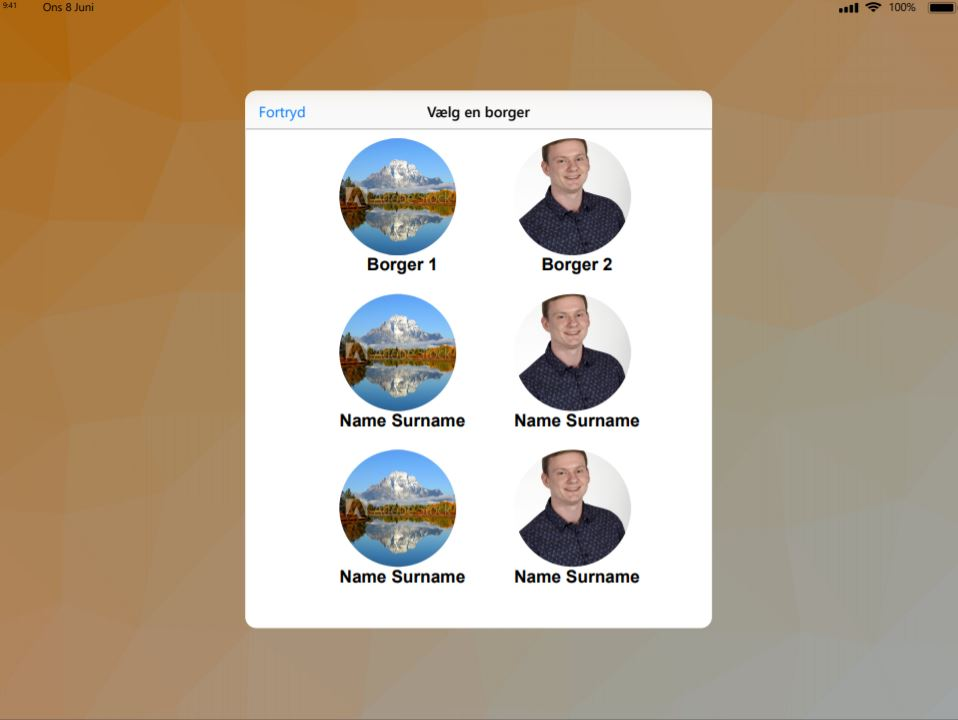
\includegraphics[width=0.8\textwidth]{figures/select-citizen.JPG}
    \caption{\label{fig:choose-citizen-prototype} Prototype of choosing a citizen.}
\end{figure}

\subsubsection{Greyscale functionality, horizontal view and how a week plan is updated}
Next the prototypes for greyscale functionality and the horizontal view of the weekplanner were shown.
Greyscale had some requested changes in the form of colors.
They would like to see a darker grey used, and the division of days should be clearer with more visible lines between days.
\\\\
The horizontal view of the weekplanner was mostly fine.
The way the names of the days were shown was not good enough, and this either needs to be redone or removed.
The main point to keep in mind with the horizontal view is that the pictogram should always be facing the right side up, which the design that was shown does.
In terms of how changes are made in the weekplanner, it was unclear whether they would make these through their own tablet or the citizen's.
Upon being posed this question, Susanne and Mette confirmed that, generally, the way it works is that they make the changes on the citizen's tablet.
Another concern is that GIRAF needs a way to display the fact that changes have been made, to avoid confusion.

\todo{Eventuelt slet horizontal mode fra listen af funktionalitet of teksten dertil længere nede.}

\subsubsection{Showing different amounts of days}
The functionality of showing different amounts of days posed some uncertainties.
GIRAF should be able to show seven days, five days, three days or just one day at a time, based on requirements defined by last year's development team.
However, if the application were to show five days ahead, and the current day were Friday, how would it handle the overlap with the next week?
This question was discussed for a while, eventually leading to the conclusion that if this were the case, they would want the program to show the next days, even if they might overlap with next week.
The problem that these days might be empty, as a plan might not have been made for the coming week, is ultimately a problem they would have to deal with on their end.

\subsubsection{Marking activities as completed, manipulating multiple activities and searching for pictograms}
In terms of marking activities as completed, they were happy with the options we presented - checkmarks, removal and greyscale.
We posed the question of how to handle removal of completed activities.
If one were to be removed upon completion, an empty space would appear on the plan - should the system account for this and automatically move all the other activities up to remove the empty space?
According to Susanne and Mette, this could cause confusion, but ultimately it would just depend on how the system was taught to the citizens.
\\\\
The ability to manipulate multiple activities at a time would be nice to have.
The prototypes we had prepared for this functionality were acceptable, however this functionality gave rise to an important discussion.
The institutions want the citizens to be as independent as possible - this means they are the ones that mark activities as completed.
Based on our impressions of the work of previous years on the GIRAF project and the prototypes that were handed down to us, we had thought the guardians would be performing this task.
On top of this, adding the ability for citizens to mark activities that were previously marked as completed as not completed would not pose a problem.
The representatives did not expect that the citizens would abuse this functionality, however they would like GIRAF to restrict this to citizens only being able to change the status of the previously completed activity.
The prototype for pictogram search was good, but they were also interested in either being able to take their own pictures to use, or to search Google for new ones, like Emil mentioned in \autoref{interview-with-emil}.

\subsubsection{The timer functionality and cancelling activities}
The timer functionality is one of the fundamental functionalities we want to add to the GIRAF project.
The requirements of the functionality were discussed alongside the prototypes.
Generally, they will add the timer as they add the activities to the week plan, rather than when the activity starts.
The only exception to this is when the citizen completely shuts down.
If this happens, they add the timer when the activity takes place, or even use a physical timer.
\\\\
The different representations of time we had designed were proposed and evaluated.
Generally they wanted to use an hourglass or a circle that gradually changed color.
When adding a timer, they would rather just input the time the activity takes in minutes rather than the time period in which the activity takes place.
Cancelling activities is a guardian only functionality, but the citizens need to be able to see that an activity has been cancelled.

\begin{figure}[h!]
  \center
  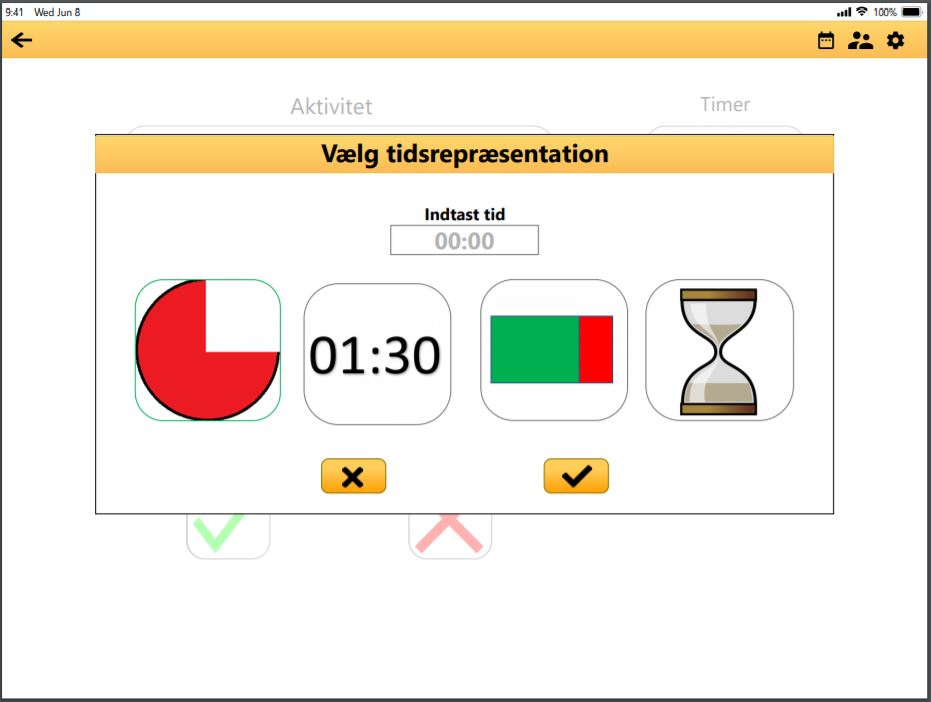
\includegraphics[width=0.8\textwidth]{figures/select-timer-prototype.JPG}
  \caption{\label{fig:choose-timer-prototype} Prototype for choosing a timer.}
\end{figure}

\subsection{The key points of the clarifying questions}
In terms of citizens having their own login or having guardians login, entering citizen mode and showing the week plan to the citizen, Susanne and Mette would like to see a login functionality specific to the citizens.
They did not think citizens being able to look at other citizen's plans would be a large issue.
When asked if the citizens were likely to use GIRAF at home, the representatives answered that this was not known.
They could receive help to plan activities for the weekend, but they will generally do different things at home compared to at the school.
In terms of the information needed for a new citizen, only names and a photo would be necessary.

\subsection{Summary of the meeting}
The most essential piece of information gained was the fact they we had misunderstood the way activities are marked as completed.
We thought the guardians would perform this action, but it is actually the citizens.
This meant the prototypes needed changing.
When selecting a citizen, an additional layer to divide them into classes would be preferable according to the representatives.
Generally, the designs proposed on the prototypes were acceptable, and the icons used were satisfactory.
